% This file was created by tikzplotlib vunknown.
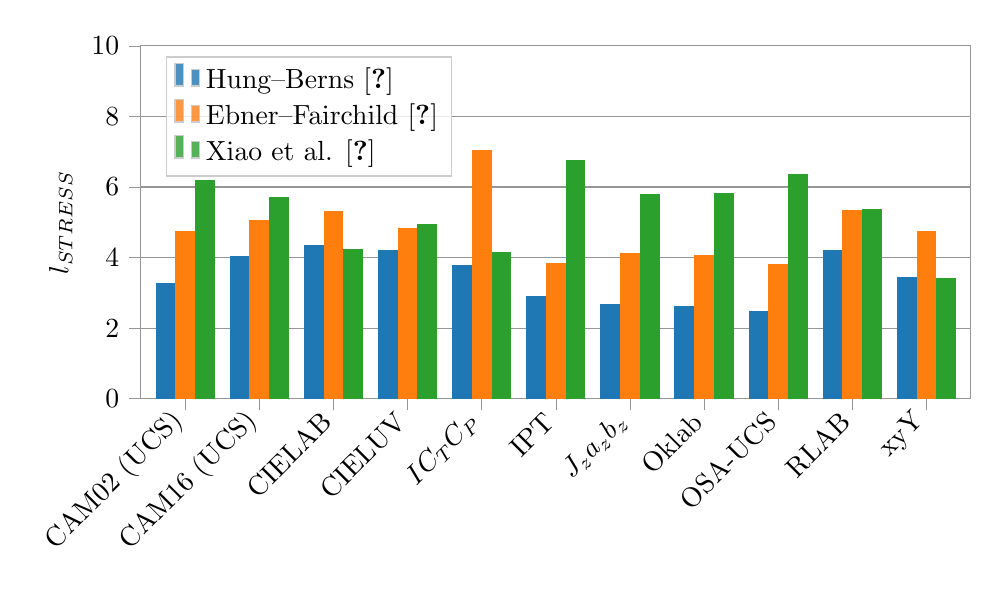
\begin{tikzpicture}

\definecolor{color0}{rgb}{0.12156862745098,0.466666666666667,0.705882352941177}
\definecolor{color1}{rgb}{1,0.498039215686275,0.0549019607843137}
\definecolor{color2}{rgb}{0.172549019607843,0.627450980392157,0.172549019607843}

\begin{axis}[
axis line style={white!58.8235294117647!black},
legend cell align={left},
width=\textwidth,
height=0.5\textwidth,
legend style={fill opacity=0.8, draw opacity=1, text opacity=1, at={(0.03,0.97)}, anchor=north west, draw=white!80!black},
tick align=outside,
tick pos=left,
x grid style={white!58.8235294117647!black},
xmin=-0.6, xmax=10.6,
xtick style={color=white!58.8235294117647!black},
xtick={0,1,2,3,4,5,6,7,8,9,10},
xticklabels={CAM02 (UCS),CAM16 (UCS),CIELAB,CIELUV,$IC_TC_P$,IPT,$J_za_zb_z$,Oklab,OSA-UCS,RLAB,xyY},
xticklabel style={rotate=45,anchor=east},
y grid style={white!58.8235294117647!black},
ylabel={$l_\text{STRESS}$},
ymajorgrids,
ymin=0, ymax=10.0,
ytick style={color=white!58.8235294117647!black}
]
\draw[draw=none,fill=color0] (axis cs:-0.4,0) rectangle (axis cs:-0.133333333333333,3.26752096358107);
\addlegendimage{ybar,ybar legend,draw=none,fill=color0};
  \addlegendentry{Hung--Berns \cite{hung}}

\draw[draw=none,fill=color0] (axis cs:0.6,0) rectangle (axis cs:0.866666666666667,4.03663610711868);
\draw[draw=none,fill=color0] (axis cs:1.6,0) rectangle (axis cs:1.86666666666667,4.34856818798823);
\draw[draw=none,fill=color0] (axis cs:2.6,0) rectangle (axis cs:2.86666666666667,4.21626028738579);
\draw[draw=none,fill=color0] (axis cs:3.6,0) rectangle (axis cs:3.86666666666667,3.7957739893557);
\draw[draw=none,fill=color0] (axis cs:4.6,0) rectangle (axis cs:4.86666666666667,2.92119683105356);
\draw[draw=none,fill=color0] (axis cs:5.6,0) rectangle (axis cs:5.86666666666667,2.68536426894407);
\draw[draw=none,fill=color0] (axis cs:6.6,0) rectangle (axis cs:6.86666666666667,2.63371950519246);
\draw[draw=none,fill=color0] (axis cs:7.6,0) rectangle (axis cs:7.86666666666667,2.49530998013144);
\draw[draw=none,fill=color0] (axis cs:8.6,0) rectangle (axis cs:8.86666666666667,4.20182174798341);
\draw[draw=none,fill=color0] (axis cs:9.6,0) rectangle (axis cs:9.86666666666667,3.44018748653443);
\draw[draw=none,fill=color1] (axis cs:-0.133333333333333,0) rectangle (axis cs:0.133333333333333,4.75235322590395);
\addlegendimage{ybar,ybar legend,draw=none,fill=color1};
  \addlegendentry{Ebner--Fairchild \cite{ebner}}

\draw[draw=none,fill=color1] (axis cs:0.866666666666667,0) rectangle (axis cs:1.13333333333333,5.07600805665883);
\draw[draw=none,fill=color1] (axis cs:1.86666666666667,0) rectangle (axis cs:2.13333333333333,5.30715095336481);
\draw[draw=none,fill=color1] (axis cs:2.86666666666667,0) rectangle (axis cs:3.13333333333333,4.82895376092783);
\draw[draw=none,fill=color1] (axis cs:3.86666666666667,0) rectangle (axis cs:4.13333333333333,7.04859738515855);
\draw[draw=none,fill=color1] (axis cs:4.86666666666667,0) rectangle (axis cs:5.13333333333333,3.8585452834895);
\draw[draw=none,fill=color1] (axis cs:5.86666666666667,0) rectangle (axis cs:6.13333333333333,4.11463844121543);
\draw[draw=none,fill=color1] (axis cs:6.86666666666667,0) rectangle (axis cs:7.13333333333333,4.05730886560147);
\draw[draw=none,fill=color1] (axis cs:7.86666666666667,0) rectangle (axis cs:8.13333333333333,3.81297237590754);
\draw[draw=none,fill=color1] (axis cs:8.86666666666667,0) rectangle (axis cs:9.13333333333333,5.35024616302759);
\draw[draw=none,fill=color1] (axis cs:9.86666666666667,0) rectangle (axis cs:10.1333333333333,4.75045818919244);
\draw[draw=none,fill=color2] (axis cs:0.133333333333333,0) rectangle (axis cs:0.4,6.20819583068419);
\addlegendimage{ybar,ybar legend,draw=none,fill=color2};
  \addlegendentry{Xiao et al. \cite{xiao}}

\draw[draw=none,fill=color2] (axis cs:1.13333333333333,0) rectangle (axis cs:1.4,5.72257615772008);
\draw[draw=none,fill=color2] (axis cs:2.13333333333333,0) rectangle (axis cs:2.4,4.23955931207367);
\draw[draw=none,fill=color2] (axis cs:3.13333333333333,0) rectangle (axis cs:3.4,4.94778942179491);
\draw[draw=none,fill=color2] (axis cs:4.13333333333333,0) rectangle (axis cs:4.4,4.1670522430841);
\draw[draw=none,fill=color2] (axis cs:5.13333333333333,0) rectangle (axis cs:5.4,6.77347388639467);
\draw[draw=none,fill=color2] (axis cs:6.13333333333333,0) rectangle (axis cs:6.4,5.79350009458213);
\draw[draw=none,fill=color2] (axis cs:7.13333333333333,0) rectangle (axis cs:7.4,5.83206308550632);
\draw[draw=none,fill=color2] (axis cs:8.13333333333333,0) rectangle (axis cs:8.4,6.37866193244541);
\draw[draw=none,fill=color2] (axis cs:9.13333333333333,0) rectangle (axis cs:9.4,5.38373889554062);
\draw[draw=none,fill=color2] (axis cs:10.1333333333333,0) rectangle (axis cs:10.4,3.40752186432328);
\end{axis}

\end{tikzpicture}
